\chapter{Vector Basics}
    \section{Recommended Texts}
        The following books are recommended for the course. The first one will be followed by the instructor.
        \begin{enumerate}
            \item Engineering Electromagnetics 8th Edition by John Buck \& William H. Hayt
            \item Electromagnetics John D. Kraus
            \item Introduction to Electrodynamics by David J. Griffiths
            \item Classical Electrodynamics by John David Jackson
        \end{enumerate}
    \section{What is a Vector?}
        From a mathematical standpoint a vector is an element of a vector space. From a physical point of view a vector is a quantity that requires a magnitude as well as a direction to be represented.
    \section{Unit vectors in Rectangular Coordinate System}
        In a Rectangular Coordinate System (RCS), a vector can be represented as a linear sum of three unit vectors, namely $\vec{a}_x$, $\vec{a}_y$ and $\vec{a}_z$. In case of two dimensions, $\vec{a}_z$ is not needed. This is also depicted in figure~\ref{fig:vectors}.
        \begin{figure}
            \centering
            \subfloat[A vector in two dimensions]{
                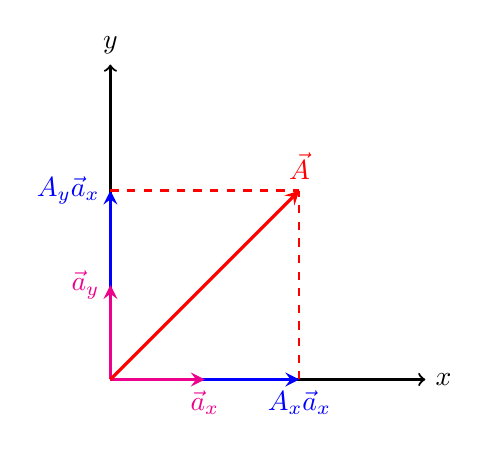
\begin{tikzpicture}
    [scale=4,
    axis/.style={->,thick},
    vector/.style={-stealth,very thick},
    vector guide/.style={dashed,red,thick}]

    \coordinate (O) at (0, 0);
    \def\u{0.3}
    \def\v{0.6}

    % drawing axes
    \draw[axis] (O) -- (1, 0) node[anchor=west]{$x$};
    \draw[axis] (O) -- (0, 1) node[anchor=south]{$y$};

    % drawing the vector's components
    \draw[vector, blue] (O) -- (\v, 0) node[anchor=north]{$A_x\vec{a}_x$};
    \draw[vector, blue] (O) -- (0, \v) node[anchor=east]{$A_y\vec{a}_x$};

    % drawing unit vectors
    \draw[vector, magenta] (O) -- (\u, 0) node[anchor=north]{$\vec{a}_x$};
    \draw[vector, magenta] (O) -- (0, \u) node[anchor=east]{$\vec{a}_y$};

    % drawing vector A
    \draw[vector, red] (O) -- (\v, \v) node[anchor=south]{$\vec{A}$};

    % drawing vector guides
    \draw[vector guide] (\v, 0) -- (\v, \v);
    \draw[vector guide] (0, \v) -- (\v, \v);

\end{tikzpicture}
            }
            \subfloat[A vector in three dimensions]{
                % sets up the perspective from which we are looking at the picture {theta}{phi}
% {theta} defines the rotion by x axis while {phi} defines the rotation by z axis
\tdplotsetmaincoords{60}{120}

\begin{tikzpicture}
    [scale=4,
    tdplot_main_coords,
    axis/.style={->,black,thick},
    vector/.style={-stealth,very thick},
    vector guide/.style={dashed,red,thick}]

    \coordinate (O) at (0, 0, 0);

    % this should serve as our unit vector
    \def\u{0.3} 
    \def\v{0.6}
    % drawing axes
    \draw[axis] (0, 0, 0) -- (1, 0, 0) node[anchor=north east]{$x$};
    \draw[axis] (0, 0, 0) -- (0, 1, 0) node[anchor=north west]{$y$};
    \draw[axis] (0, 0, 0) -- (0, 0, 1) node[anchor=south]{$z$};

    % drawing the components of the vector A: Drawing them first so the unit vectors do appear
    \draw[vector, blue] (O) -- (\v, 0, 0) node[anchor=south east]{$B_x\vec{a}_x$};
    \draw[vector, blue] (O) -- (0, \v, 0) node[anchor=south west]{$B_y\vec{a}_y$};
    \draw[vector, blue] (O) -- (0, 0, \v) node[anchor=south east]{$B_z\vec{a}_z$};

    % drawing the unit vectors
    \draw[vector, magenta] (O) -- (\u, 0, 0) node[anchor=south east]{$\vec{a}_x$};
    \draw[vector, magenta] (O) -- (0, \u, 0) node[anchor=south west]{$\vec{a}_y$};
    \draw[vector, magenta] (O) -- (0, 0, \u) node[anchor=east]{$\vec{a}_z$};

    % drawing the main vector B
    \draw[vector, red] (O) -- (\v, \v, \v) node[anchor=south east]{$\vec{B}$};

    % projection on xy axis
    \draw[vector guide] (\v, 0, 0) -- (\v, \v, 0);
    \draw[vector guide] (0, \v, 0) -- (\v, \v, 0);
    \draw [vector guide] (\v, \v, 0) -- (\v, \v, \v);

    % drawing projection on yz axis
    \draw[vector guide] (0, \v, 0) -- (0, \v, \v);
    \draw[vector guide] (0, 0, \v) -- (0, \v, \v);
    \draw[vector guide] (0, \v, \v) -- (\v, \v, \v);

    % drawing projection on xz axis
    \draw[vector guide] (0, 0, \v) -- (\v, 0, \v);
    \draw[vector guide] (\v, 0, 0) -- (\v, 0, \v);
    \draw[vector guide] (\v, 0, \v) -- (\v, \v, \v);


\end{tikzpicture}
            }
            \caption{}
            \label{fig:vectors}
        \end{figure}
    \section{Dot Product}
        Suppose we have two vectors $\vec{A}$ and $\vec{B}$. $\vec{A}$ can be represented as:
        $$\vec{A} = A_x\vec{a}_x + A_y\vec{a}_y + A_z\vec{a}_z$$
        Similarly, $\vec{B}$ can be represented as:
        $$\vec{B} = B_x\vec{a}_x + B_y\vec{a}_y + B_z\vec{a}_z$$
        Their dot product, $\vec{A}\cdot \vec{B}$, which is a scalar quantity, is defined as:
        $$\vec{A}\cdot \vec{B} = |\vec{A}||\vec{B}|\cos \theta$$
        In case when $\theta$ becomes $90^{\circ}$ the dot product automatically reduces to zero. Thus one can easily conclude that the dot product of two perpendicular vectors shall always be zero. This makes expressing the dot product in terms of its components pretty straight forward.
        $$\vec{A}\cdot \vec{B} = \left(A_x\vec{a}_x + A_y\vec{a}_y + A_z\vec{a}_z\right)\cdot \left(B_x\vec{a}_x + B_y\vec{a}_y + B_z\vec{a}_z\right)$$
        \begin{equation}\label{eq:dotproduct}
           \vec{A}\cdot \vec{B} = A_xB_x + A_yB_y + A_zB_z
        \end{equation}
        A vector can also be represented in the form of column vector as:
        $$ \vec{A} = \begin{bmatrix}A_x \\A_y \\A_z\\ \end{bmatrix} \quad \vec{B} = \begin{bmatrix}B_x \\B_y \\B_z\\ \end{bmatrix} $$
        In that case the dot product, also called inner product in this context, is defined as:
        $$ \mathbf{A}^{T}\mathbf{B} $$
        If the vectors $\vec{A}$ and $\vec{B}$ are of the order $n \times 1$ their inner product will have the order $ 1 \times \left(n \times n\right) \times 1 = 1 \times 1$. Thus the result will be a scalar quantity.
        The opposite of the inner product is known as the outer product also called the cross product which we will get to in a later topic.
        
        \subsection{Cauchy Bunyakovsky Schwarz Inequality}
            The theorem states:
            $$|\vec{A}\cdot \vec{B}| \leq |\vec{A}||\vec{B}|$$
            It's easy to see why this is the case by replacing $\vec{A}\cdot \vec{B}$ by it's value:
            $$|\vec{A}||\vec{B}|\cos \theta \leq |\vec{A}||\vec{B}| $$
            This inequality changes to an equality when both vectors are collinear.
        
        \subsection{The Triangle Inequality}
            $$|\vec{A}| + |\vec{B}| \geq |\vec{A} + \vec{B}| $$
            It's quite easy to see why that is the case in the case of two dimensions.
            At this moment it should be useful to point out that:
            $$|\vec{A}| = \sqrt{A_x^2 + A_y^2 + A_z^2}$$
            $$|\vec{A}|^2 = \vec{A} \cdot \vec{A}$$
            This shall be useful in proving the Parallelogram Equality.
        
        \subsection{The Parallelogram Equality}
            The equality states:
            $$|\vec{A} + \vec{B}|^2 + |\vec{A} - \vec{B}|^2 = 2\left(|\vec{A}|^2+\vec{B}^2\right)$$
            To prove it:
            $$|\vec{A} + \vec{B}|^2 = \left(\vec{A}+\vec{B}\right)\cdot \left(\vec{A}+\vec{B}\right)$$
            $$= \vec{A}\cdot \vec{A} + \vec{A}\cdot \vec{B} + \vec{B}\cdot \vec{A} + \vec{B}\cdot \vec{B}$$
            $$= |\vec{A}|^2 -2\vec{A}\cdot \vec{B} + |\vec{B}|^2$$
            Similarly:
            $$|\vec{A} - \vec{B}|^2 = \left(\vec{A}-\vec{B}\right)\cdot \left(\vec{A}-\vec{B}\right)$$
            $$= \vec{A}\cdot \vec{A} - \vec{A}\cdot \vec{B} - \vec{B}\cdot \vec{A} + \vec{B}\cdot \vec{B}$$
            $$= |\vec{A}|^2 +2\vec{A}\cdot \vec{B} + |\vec{B}|^2$$
            Thus:
            $$|\vec{A} + \vec{B}|^2 + |\vec{A} - \vec{B}|^2 = 2|\vec{A}| + 2|\vec{B}| = 2\left(|\vec{A}| + |\vec{B}|\right)$$
        
        \subsection{Some practical applications}
            Some common places in Physics where you will find the dot product being applied are:
            \begin{itemize}
                \item The formulas for work done.
                        $$W = \vec{F}\cdot \vec{d}$$ 
                        $$dW = \vec{F}\cdot \vec{dl}$$
                        $$W = \int\limits_{L} \vec{F}\cdot \vec{dl}$$
                \item The forumulas for Electric and Magnetic flux.
                        $$\phi_E = \vec{E}\cdot \vec{A}$$
                        $$\phi_M = \vec{B}\cdot \vec{A}$$
                \item A third one I don't understand yet. Need to confirm this one.
                        $$Q = \iint\limits_{S}\vec{D}\cdot \vec{dS}$$
            \end{itemize}
    \section{Cross Product}
        \subsection{The Definition}
            The cross product of two vectors $\vec{A}$ and $\vec{B}$ is given by:
            \begin{equation}\label{eq:crossproduct}
                \vec{A}\times \vec{B} = |\vec{A}||\vec{B}|\sin\theta \vec{u}_N
            \end{equation}
            Where $\theta\in\left[0, \pi\right]$ and $\vec{u}_N$ is a vector given by the right hand rule where fingers should be curled from the direction of $\vec{A}$ to the direction of $\vec{B}$.
            Since the direction of the cross product is dictated by the right hand rule we can already see that it is not a commutative operation. More accurately:
            \begin{equation}\label{eq:commutativeincrossproduct}
                \vec{A}\times\vec{B} = - (\vec{B}\times\vec{A})
            \end{equation}
            
        \subsection{Geometric Significance}
            \begin{figure}
    \centering
    \begin{tikzpicture}
        [scale=4,
        axis/.style={->,thick},
        vector/.style={-stealth,very thick},
        vector guide/.style={dashed,red,thick}]

        % drawing both vectors and their angle's arc
        \draw[vector, blue] (0, 0) -- (0.5, 0) node[anchor=north]{$\vec{A}$};
        \draw[vector, red] (0, 0) -- (30: 0.5) node[anchor=south]{$\vec{B}$};
        \draw[black] (0.1, 0) arc (0:30:0.1);
        \draw (12: 0.2) node[anchor=east]{$\theta$};

        % drawing the other lines 
        \draw[black, very thick] (30: 0.5) -- ++(0.5, 0);
        \draw[black, very thick] (0.5, 0) -- ++(30: 0.5);

        % height of the parallelogram
        \draw[dashed] (30:0.5) -- node[left]{$h$} ($(0,0)!(30:0.5)!(1,0)$);
    \end{tikzpicture}
    \caption{A parallelogram formed by two vectors $\vec{A}$ and $\vec{B}$}
    \label{fig:parallelogram}
\end{figure}
            As you can see very clearly in figure~\ref{fig:parallelogram} that any two vectors $\vec{A}$ and $\vec{B}$ can uniquely identify a parallelogram. The area of any parallelogram is given by the formula:
            \begin{equation}\label{eq:areaofparallelogram}
            Area = (base)\times(height)
            \end{equation}
            In figure~\ref{fig:parallelogram} the base is the length of the vector $\vec{A}$ and the height is shown by the dotted line. But how do we figure out what $h$ really is? By applying trigonometry here we can find out that $h = |\vec{A}|\sin\theta$. Plugging in these values in equation~\ref{eq:areaofparallelogram} we get:
            $$Area = (|\vec{B}|)(|\vec{A}|\sin\theta)$$
            Ahah, this is exactly the same formula that is given by $\vec{A}\cdot\vec{B}$. Thus we can conclude that the area of the parallelogram formed by two vectors $\vec{A}$ and $\vec{B}$ is given by $\vec{A}\cdot\vec{B}$.
            $$Area = \vec{A}\cdot\vec{B}$$
        
        \subsection{Calculating Cross Product}
            Before we learn how to calculate the cross product of any two vectors in terms of the three basic unit vectors $\vec{a}_x$, $\vec{a}_y$ and $\vec{a}_z$ we should think about what will be the cross production of every possible combination of two of these three unit vectors. We know from equation~\ref{eq:crossproduct} that the cross product of two parallel vectors should be zero because $\sin 90^{\circ} = 0$. We also know that the magnitude of a unit vector is by definition one. Using these two facts, along with the right hand rule, we can very quickly see that:
            $$\vec{a}_x\times\vec{a}_y=\vec{a}_z$$
            $$\vec{a}_y\times\vec{a}_z=\vec{a}_x$$
            $$\vec{a}_z\times\vec{a}_x=\vec{a}_y$$
            Using equation~\ref{eq:commutativeincrossproduct} we can easily figure out the reverses of these combinations:
            $$\vec{a}_y\times\vec{a}_x=-\vec{a}_z$$
            $$\vec{a}_z\times\vec{a}_y=-\vec{a}_x$$
            $$\vec{a}_x\times\vec{a}_z=-\vec{a}_y$$
            Now suppose we have two vectors $\vec{A}$ and $\vec{B}$, we can express them as:
            $$\vec{A} = A_x\vec{a}_x + A_y\vec{a}_y + A_z\vec{a}_z$$
            $$\vec{B} = B_x\vec{a}_x + B_y\vec{a}_y + B_z\vec{a}_z$$
            Their cross product can be written as:
            $$\vec{A}\times\vec{B} = \left(A_x\vec{a}_x + A_y\vec{a}_y + A_z\vec{a}_z\right)\times\left(B_x\vec{a}_x + B_y\vec{a}_y + B_z\vec{a}_z\right)$$
            Expanding this we get:
            \begin{align*}
            \vec{A}\times\vec{B} = A_xB_x(\vec{a}_x\times\vec{a}_x) + A_xB_y(\vec{a}_x\times\vec{a}_y) + A_xB_z(\vec{a}_x\times\vec{a}_z)\\ + A_yB_x(\vec{a}_y\times\vec{a}_x) + A_yB_y(\vec{a}_y\times\vec{a}_y) + A_yB_z(\vec{a}_y\times\vec{a}_z)\\ + A_zB_x(\vec{a}_z\times\vec{a}_x) + A_zB_y(\vec{a}_z\times\vec{a}_y) + A_zB_z(\vec{a}_z\times\vec{a}_z)
            \end{align*}
            Firstly, we can cancel those cross products which are between collinear vectors, as we know that's going to be zero.
            \begin{align*}
            \vec{A}\times\vec{B} = A_xB_y(\vec{a}_x\times\vec{a}_y) + A_xB_z(\vec{a}_x\times\vec{a}_z)\\ + A_yB_x(\vec{a}_y\times\vec{a}_x)  + A_yB_z(\vec{a}_y\times\vec{a}_z)\\ + A_zB_x(\vec{a}_z\times\vec{a}_x) + A_zB_y(\vec{a}_z\times\vec{a}_y) 
            \end{align*}
            Now, just utilizing the crossproducts of all possible combinations between unit vectors that we just derived a while ago, we can simplify this even further:
            \begin{align*}
            \vec{A}\times\vec{B} = A_xB_y(\vec{a}_z) + A_xB_z(-\vec{a}_y)\\ + A_yB_x(-\vec{a}_z)  + A_yB_z(\vec{a}_x)\\ + A_zB_x(\vec{a}_y) + A_zB_y(-\vec{a}_x) 
            \end{align*}
            Grouping these terms by unit vectors we get:
            \begin{equation}
                \vec{A}\times\vec{B} = \vec{a}_x(A_yB_z-A_zB_y) + \vec{a}_y(A_zB_x-A_xB_z) + \vec{a}_z(A_xB_y-A_yB_x)
            \end{equation}
            We can write this in an elegant way as a determinant:
            \begin{equation}
                \vec{A}\times\vec{B} = \begin{vmatrix}
                    \vec{a}_x & \vec{a}_y & \vec{a}_z \\
                    A_x & A_y & A_z\\
                    B_x & B_y & B_z
                \end{vmatrix}
            \end{equation}
